\documentclass[11pt]{amsart}
\usepackage{geometry}                % See geometry.pdf to learn the layout options. There are lots.
\geometry{letterpaper}                   % ... or a4paper or a5paper or ... 
%\geometry{landscape}                % Activate for for rotated page geometry
%\usepackage[parfill]{parskip}    % Activate to begin paragraphs with an empty line rather than an indent
\usepackage{graphicx}
\usepackage{amssymb}
\usepackage{epstopdf}
\usepackage{amsthm}
\usepackage{enumerate}
%\DeclareGraphicsRule{.tif}{png}{.png}{`convert #1 `dirname #1`/`basename #1 .tif`.png}
\setlength{\parindent}{0em}
\setlength{\parskip}{1em}
\newtheorem{defn}{Definition}
\newtheorem{thm}{Theorem}

\begin{document}
\begin{center}
\bigskip 
\textbf{Envelopes, Support Functions and the Convex Hull}

\textsc{Jeffrey Rosenbluth}

\textit{April 2015}
\end{center}
\hrule
\vspace{0.25in}

We define both envelopes and convex hulls in terms of \emph{support functions} and show
that the convex hull is a (possibly proper) subset of the envelope. It turns out that our notion of
envelope is intimately related to the diagram's support function as we will make precise below.
In fact if we restrict ourselves to normalized vectors (there is no harm in doing this since the envelope
is really a function of direction), then there is no difference between the two concepts.
Finally we make some observations about envelopes. 

\section{Envelope vs Convex Hull}

We start with the definition of support functions
on  $\mathbb{R}^n$.\footnote{
The definition of a support function can be generalized to arbitrary normed linear spaces over the reals.
Let $S$ be any set in a vector space $X$. We define the support function $q_S$ on the dual $X'$ of $X$ as 
$q_S(\ell) = sup_{s \in S} \ell(s)$
for any linear function $\ell.$ 
(see \emph{Functional Analysis}, by Peter Lax, 2002, p. 84).
}
\begin{defn}[Support Function]
\label{supportfunc}
Let $S$ be a set in $\mathbb{R}^n$. We define the support function $q_S$ as 
$$q_S(v) = sup_{s \in S} \langle s,v \rangle$$
where $\langle \cdot, \cdot \rangle$ denotes inner product.
\end{defn}

Note that $q_S(v)$ may be $\infty$ for some $v$. The following theorem
and example will help us gain some intuition about support functions.\footnote{The proof of the theorem can
be found in \emph{Convex Sets and Their Applications} by Steven R Lay, 1982. pp. 206-207.} 

\begin{thm}
Let $S$ be a nonempty compact convex set and let $q$ be its support function. If $v$ is any fixed point other
than the origin, then the following hold:
\begin{enumerate}[i.]
\item There exists a point $x_v$ in $S$ such that $q(v)=\langle x_v, v \rangle$.
\item The hyperplane $H \equiv \{x : \langle x, v \rangle = q(v)\}$ supports $S$ at $x_v$.
\item The signed distance from $H$ to the origin is $q(v/\|v\|)$.
\end{enumerate}
\end{thm}

\textsc{Example}. Let $d$ be the diamond in $\mathbb{R}^2$ with vertices $(0, \pm1)$ and $(\pm 1, 0)$ (see Figure 1). To calculate $q(v)$ for $v = (2,1)$ 
we need to calculate $sup_{s \in d} \langle s, v \rangle$. This maximum is easily seen to be attained at the point $(1,0)$ and hence $q(v) = \langle (1,0),(2,1) \rangle = 2$. In
general we have $q((x,y)) = \max(|x|,|y|)$.

\begin{figure}[h]
\label{diamond}
\centering
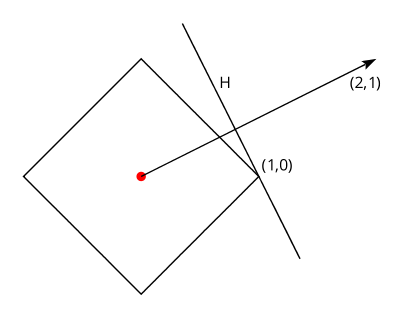
\includegraphics[width=150pt]{diamond.png}
\caption{diamond}
\end{figure}

In contrast to diagrams we will not distinguish between points and vectors, taking the definition of both to be elements in $\mathbb{R}^n$.
This allows us to fix the origin at $0$ and to consider two diagrams that are identical except for their origins to be translations of one another.

From the diagrams documentation and Definition \ref{supportfunc} we can rewrite the definition of an envelope 
in terms of its support function $q_d$.
\begin{defn}[Envelope]
The envelope of a diagram $d$ in direction $v$ is
\begin{align}
e_d(v) &= sup_{u \in d} \frac{\langle u, v \rangle}{\|v\|^2}\\
           &=sup_{u \in d} \langle u, v/\|v\|^2 \rangle\\
           &=q_d(v/\|v\|^2)
\end{align}
\end{defn}

We can create an intensional representation of the envelope by taking the union over all $v$ of the sets
$$\{av : a \leq e_d(v)\} \cap \{ bv : b \leq e_d(-v)\}$$
Therefore if we can represent the convex hull as the union over all $v$ of the sets
$$\{av : a \leq c_d(v)\} \cap \{ bv : b \leq c_d(-v)\}$$
where $c_d(v) \leq e_d(v)$, then we will have shown the convex hull of $d$ is a subset of its envelope.

To define the convex hull in terms of the support function we use the following theorem. 
\footnote{\emph{Linear Algebra}, by Peter Lax, 1997, page 162. This theorem can also be generalized to
arbitrary normed linear spaces over $\mathbb{R}$. It is interesting to note that the proof of the general case requires
Zorn's lemma - which is equivalent to the axiom of choice.}

\begin{thm}[Convex Hull]
\label{convexhull} The closed convex hull of any set $S$ is the set of points x satisfying $\langle u, x \rangle \leq q_S(u)$ for all $u$ in $\mathbb{R}^n$.
\end{thm}

\begin{thm}
The convex hull of a diagram is a subset of its envelope
\end{thm}
\textsc{Proof}: We consider all points in the convex hull of diagram $d$ that lie on some vector $v$, these points have the form $c_d(v)v$ for some
scalar $c_d(v)$. By Theorem \ref{convexhull}, for all $u$, these points must satisfy
\begin{align}
\langle u, c_d(v)v \rangle &\leq q_d(u)\\
c_d(v)\langle u, v \rangle &\leq q_d(u)\\
c_d(v) &\leq  \frac{q_d(u)}{\langle u, v \rangle}
\end{align}
Since the last inequality holds for all $u$ we have,
\begin{align}
c_d(v) &= \inf_{u \in \mathbb{R}^n}  \frac{q_d(u)}{\langle u, v \rangle}\\
&\leq \frac{q_d(v)}{\langle v, v \rangle} \\
&= q_d(v/\|v\|^2)= e_d(v) 
\end{align}
 and hence $c_d(v) \leq e_d(v)$ which is suffiicient to prove the Theorem as explained above. \qed
 
 Finally, in order to show that the convex hull may be a proper subset of the envelope it is enough to find some diagram $d$ and vector $v$ such that
 $c_d(v) < e_d(v)$. We take $d$ equal to the horizontal line from $(0,0)$ to $(1,0)$ in $\mathbb{R}^2$ and $v=(1,1)$. Then
 \begin{align}
 e_d((1,1)) &= sup_{x \in [0,1]} \frac{\langle (x,0), (1,1) \rangle}{2}\\
                 &= sup_{x \in [0,1]} \frac{x}{2}\\
                 &= \frac{1}{2}
\end{align}
The convex hull of $d$ is $d$ since a line segment is convex, and the only point in $d$ lying on $(1,1)$ is $(0,0)$, hence $c_d((1,1)) = 0$ which is less than 
$1/2$, thus $c_d((1,1)) < e_d((1,1))$.

\section{Observations}

Almost all diagrams have an envelope which is a proper subset of its convex hull, Figures 2,3 and 6.
In some cases the bounding box is a better approximation to the convex hull than the envelope, a square
for example.

\begin{figure}[h]
\label{s00}
 \centering
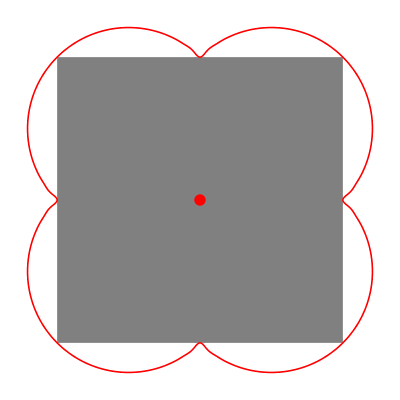
\includegraphics[width=150pt]{sq1_0_0.png}
\caption{Envelope of unit square centered at $(0,0)$}
\end{figure}

\begin{figure}[h]
\label{s05}
 \centering
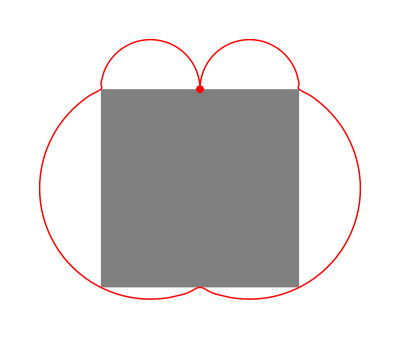
\includegraphics[width=150pt]{sq1_05.png}
\caption{Envelope of unit square centered at $(0,-\frac{1}{2})$}
\end{figure}

The envelope of a diagram is highly dependent on its origin, Figures 4 and 5.
As the origin moves farther away from the center of the diagram, the envelope becomes a 
worse approximation to the convex hull.

\begin{figure}[h]
\label{s55}
 \centering
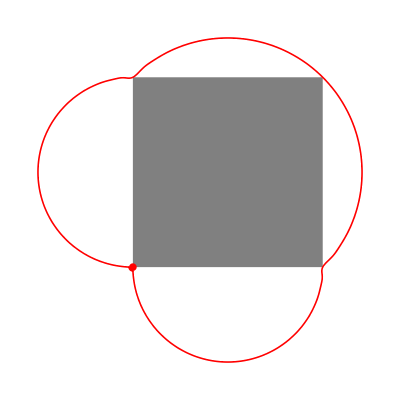
\includegraphics[width=150pt]{sq1_55.png}
\caption{Envelope of unit square centered at $(\frac{1}{2}, \frac{1}{2})$}
\end{figure}

\begin{figure}[h]
 \centering
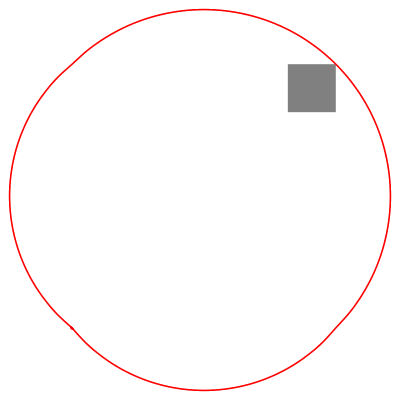
\includegraphics[width=150pt]{sq1_11.png}
\caption{Envelope of unit square centered at $(5,5)$}
\end{figure}

\begin{figure}[h]
 \centering
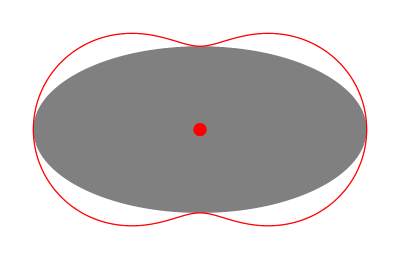
\includegraphics[width=150pt]{c1_00.png}
\caption{Envelope of an ellipse}
\end{figure}

Like the convex hull the shape of the bounding box is independent of the placement of the origin. This is not true of envelopes.
Finally, I wonder if there is an efficient algorithm to calculate and extensional form of the convex hull using the variational form
$$c_d(v) = \inf_{u \in \mathbb{R}^n}  \frac{q_d(u)}{\langle u, v \rangle}$$

\end{document}  